\documentclass[10pt, compress]{beamer}

\usetheme{m}

\usepackage{booktabs}
\usepackage[scale=2]{ccicons}

%Icons
\usepackage{fontawesome}

%Syntax highlight
\usepackage{listings,xcolor}
\usepackage{inconsolata}

\definecolor{dkgreen}{rgb}{0,.6,0}
\definecolor{dkblue}{rgb}{0,0,.6}
\definecolor{dkyellow}{cmyk}{0,0,.8,.3}

% Language: PHP
\lstset{
  language        = php,
  basicstyle      = \small\ttfamily,
  keywordstyle    = \color{dkblue},
  stringstyle     = \color{red},
  identifierstyle = \color{dkgreen},
  commentstyle    = \color{gray},
  emph            =[1]{php},
  emphstyle       =[1]\color{black},
  emph            =[2]{if,and,or,else},
  emphstyle       =[2]\color{dkyellow}}

\usepgfplotslibrary{dateplot}


\title{SMT in reverse engineering, for dummies}	
%\subtitle{}
\date{\today}
\author{Carl Svensson}
\institute{SEC-T 2016}

\begin{document}

\maketitle

\begin{frame}{About me}
  
	\begin{columns}
		\begin{column}{0.6\textwidth}  
  
  		\begin{itemize}
		  \item Carl Svensson, 25
		  \item MSc in Computer Science, KTH
		  \item IT Security consultant, Bitsec AB
		  \item CTF-player, HackingForSoju
		  \item \faEnvelope \hskip 2mm calle.svensson@zeta-two.com
		  \item \faTwitter \hskip 2mm  @zetatwo
		  \item \faGlobe \hskip 2mm https://zeta-two.com
		\end{itemize}
		
		\end{column}
		\begin{column}{0.4\textwidth} 
			\begin{center}
			
\includegraphics[width=0.4\textwidth]{images/kth.jpg}
			\end{center}
			\vspace{1cm}
			
\includegraphics[width=\textwidth]{images/bitsec.jpg}
		\end{column}
	\end{columns}
  
\end{frame}

\begin{frame}{Reverse engineering in 15 seconds?}

 \begin{itemize}
  \item Take stuff, e.g. software, apart
  \item Understand how it works
  \item Many possible goals
  \begin{itemize}
  	\item How can I reach a specific state?
  \end{itemize}  
  \end{itemize}    

\end{frame}

\begin{frame}{What is SMT?}

  \begin{itemize}
  \item Satisfiability modulo theories, SMT
  \item A bunch of variables
  \item A bunch of theories
  \begin{itemize}
    \item Theory = A bunch of rules
  \end{itemize}  
  \item A bunch of formulas
  \item Can we find values for all values s.t. all formulas are satisifed?
  \end{itemize}   

\end{frame}

\begin{frame}{SMT: Example 1}

	\begin{columns}
		\begin{column}{0.7\textwidth}
			\huge{$ x+13=37 $}
		\end{column}
		\begin{column}{0.3\textwidth}
			
\includegraphics[width=0.8\textwidth]{images/happy.png}
		\end{column}
	\end{columns}
 
\end{frame}

\begin{frame}{SMT: Example 2}

	\begin{columns}
		\begin{column}{0.7\textwidth}
			\huge{$ x+y+13=37-z $} \\
			\huge{$ x-2 \cdot y+10=10 \cdot z $} \\
			\huge{$ 4\cdot x-z+13=37+y $} \\
		\end{column}
		\begin{column}{0.3\textwidth}
			
\includegraphics[width=0.8\textwidth]{images/thinking.png}
		\end{column}
	\end{columns} 
	
\end{frame}

\begin{frame}{SMT: Example 3}

	\begin{columns}
		\begin{column}{0.7\textwidth}
			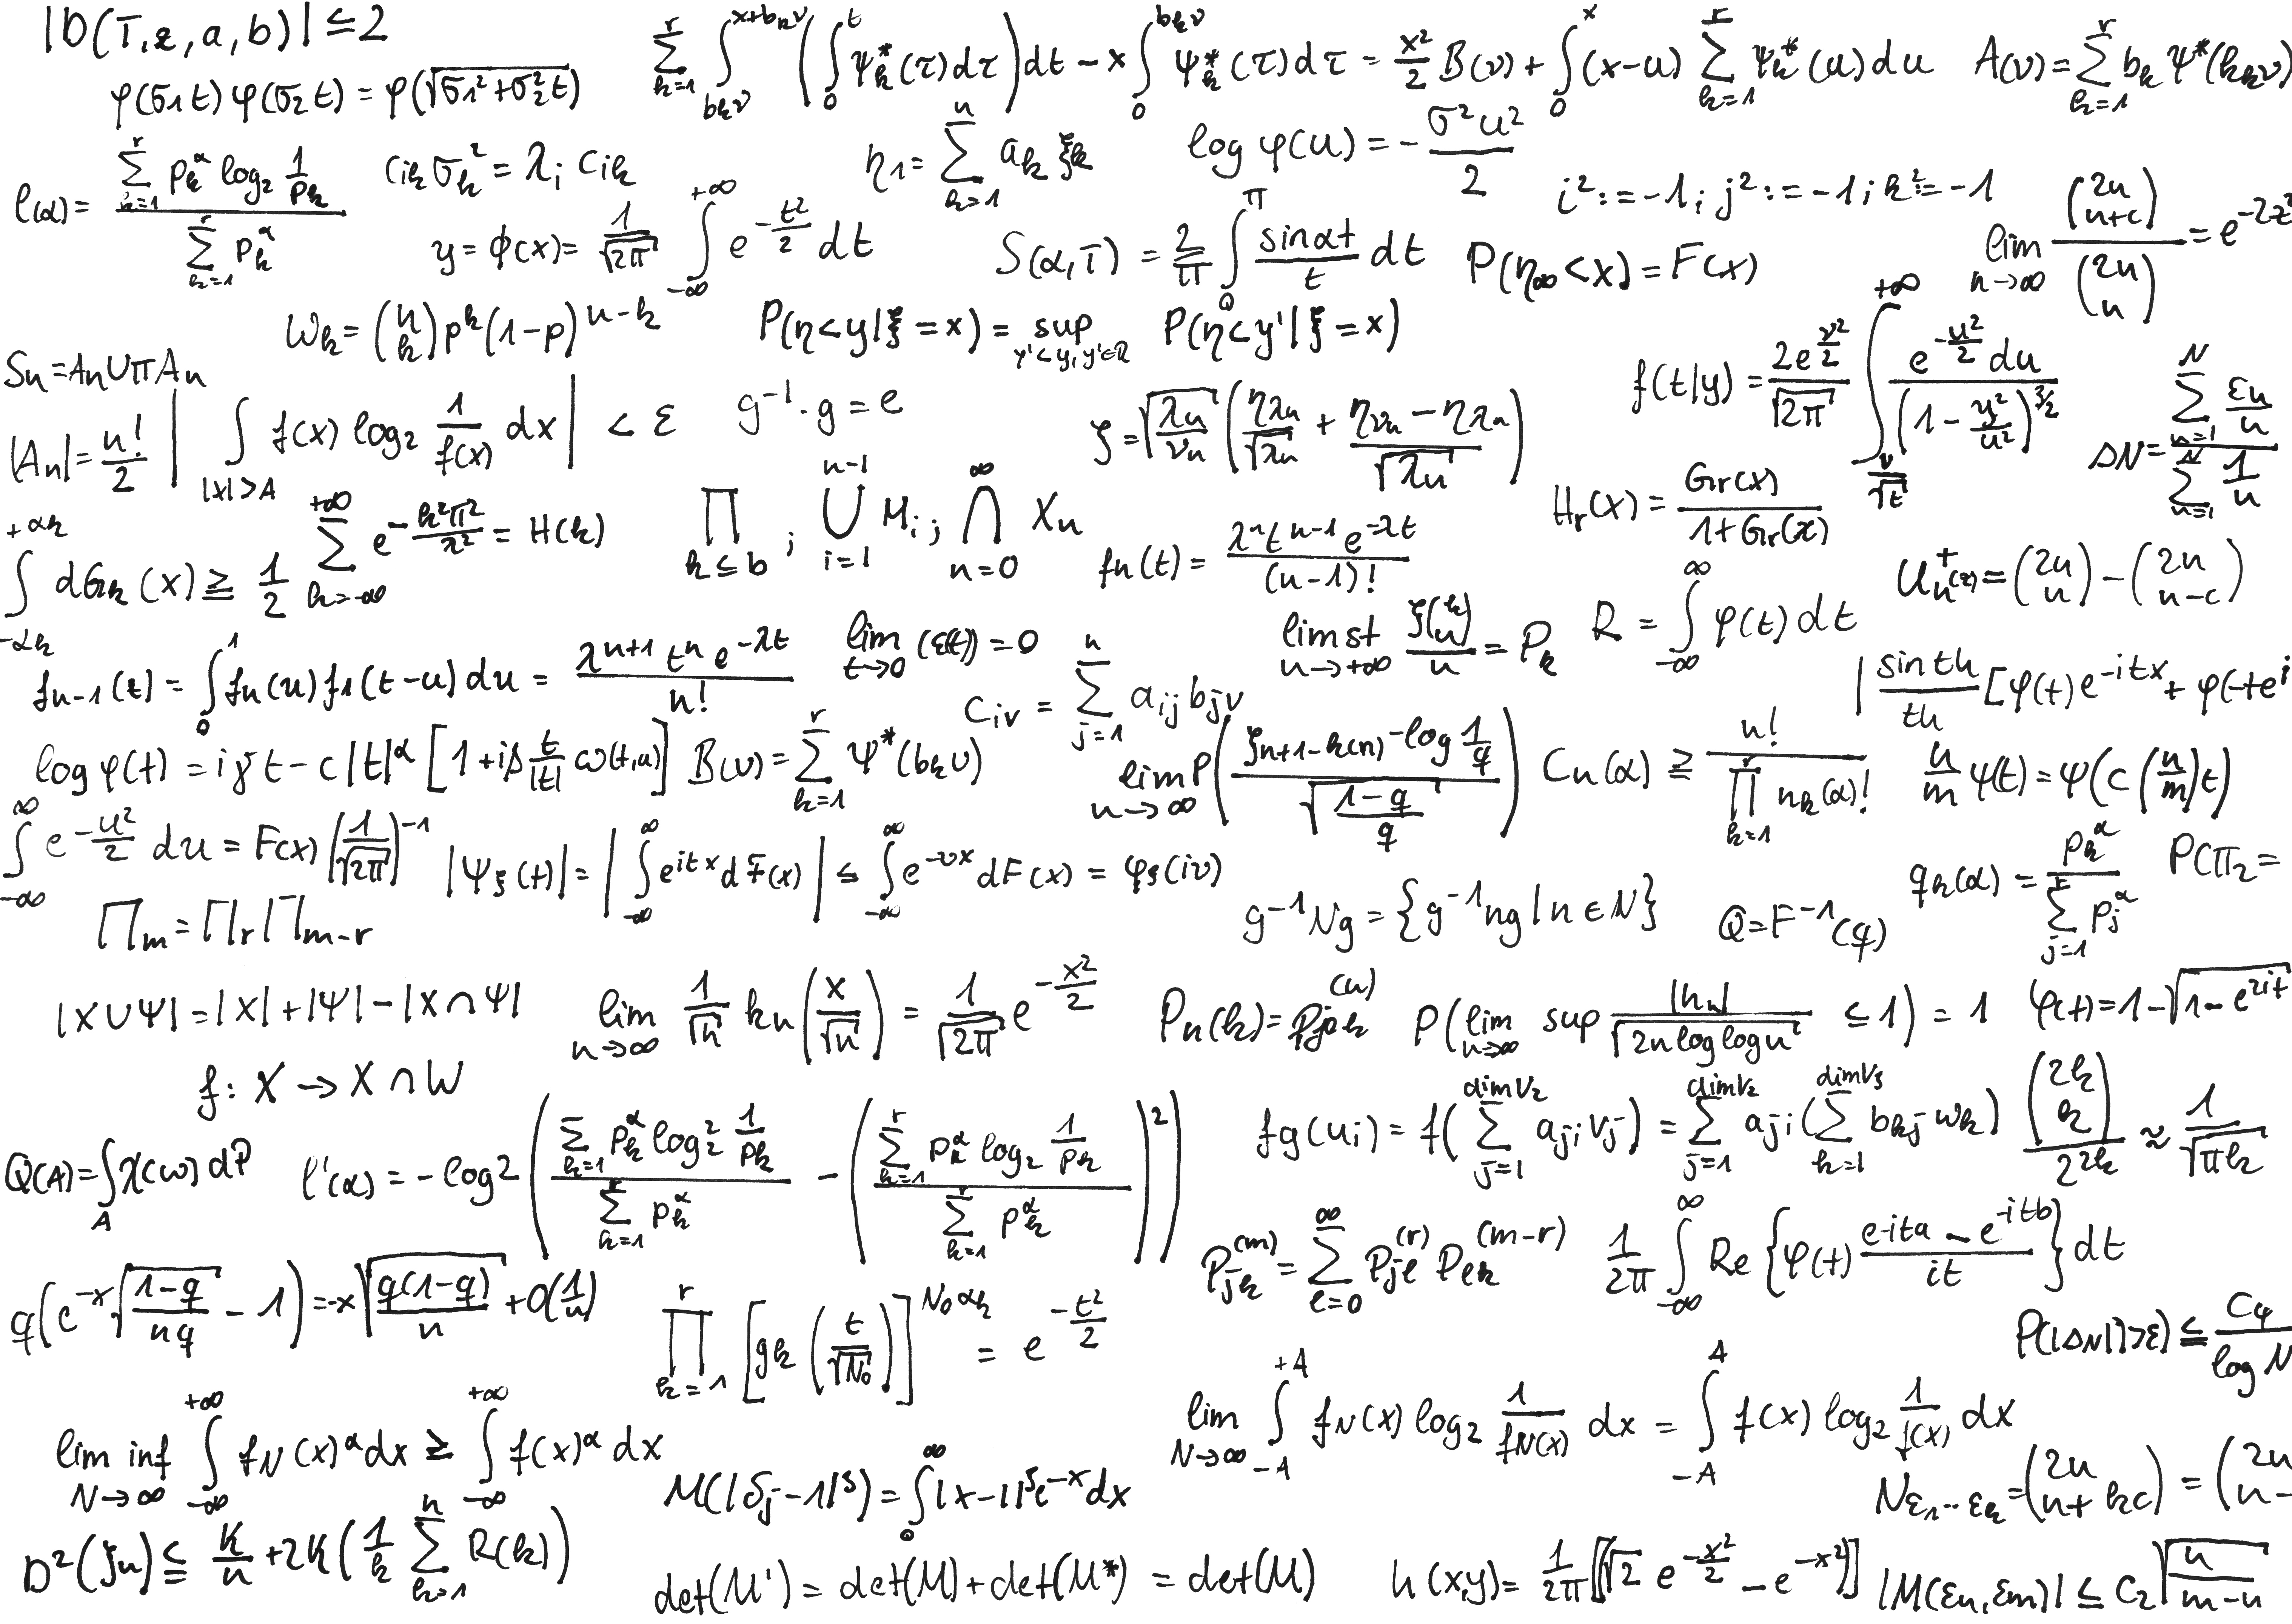
\includegraphics[width=\textwidth]{images/equations.jpg}
		\end{column}
		\begin{column}{0.3\textwidth}
			
\includegraphics[width=0.8\textwidth]{images/angry.png}
		\end{column}
	\end{columns}  
	
\end{frame}


\begin{frame}{Microsoft to the rescue}

	\begin{columns}
		\begin{column}{0.6\textwidth}

		\begin{itemize}
		\item Can we automate? Yes!
		\item Microsoft Research
		\item Z3 Theorem Prover
		\begin{itemize}
			\item General purpose
			\item Own language
			\item Bindings for several languages
			\item Open source \& cross platform
		\end{itemize}   
		\end{itemize}   
		
		\end{column}
		\begin{column}{0.4\textwidth}
			
\includegraphics{images/z3-logo.png}
		\end{column}
	\end{columns}		

\end{frame}

\begin{frame}{Using Z3 in RE}
\section{Throwback Thursday: Starcraft}
\end{frame}

\begin{frame}{Throwback Thursday: Starcraft}


	\begin{columns}
		\begin{column}{0.4\textwidth}
			\begin{itemize}
			\item Commercial software
			\item Released in 1998
			\begin{itemize}
				\item Simple protections
				\item Good starting point
			\end{itemize}
			\item Requires a serial key
			\item Can we create our own?
		\end{itemize}
		\end{column}
		\begin{column}{0.6\textwidth}
			
\includegraphics[width=\textwidth]{images/starcraft.jpg}
		\end{column}
	\end{columns}

	
\end{frame}

\begin{frame}{Getting to the core: Installer}
	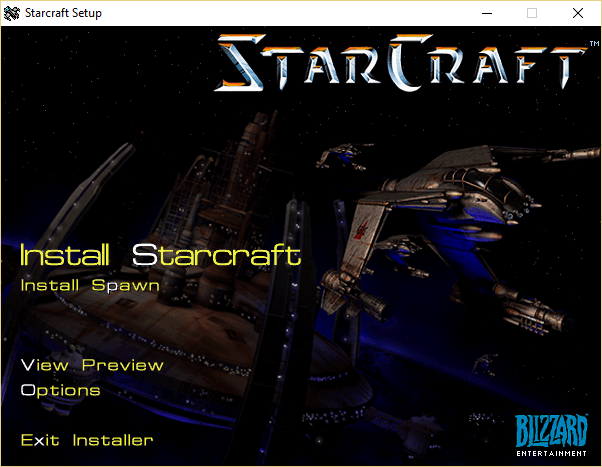
\includegraphics[width=0.8\textwidth]{images/sc1-1-setup.png}
\end{frame}

\begin{frame}{Getting to the core: Serial key input}
	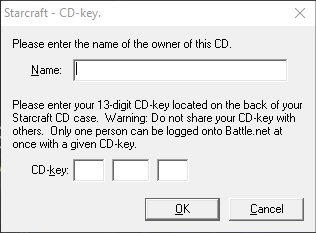
\includegraphics[width=0.9\textwidth]{images/sc1-2-input-key.png}
\end{frame}

\begin{frame}{Getting to the core: Resource strings}
	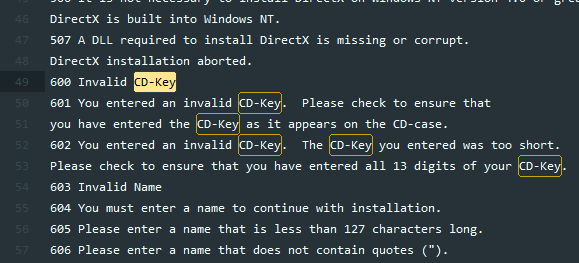
\includegraphics[width=\textwidth]{images/sc1-3-resources-strings.png}
\end{frame}

\begin{frame}{Getting to the core: Decompilation}
	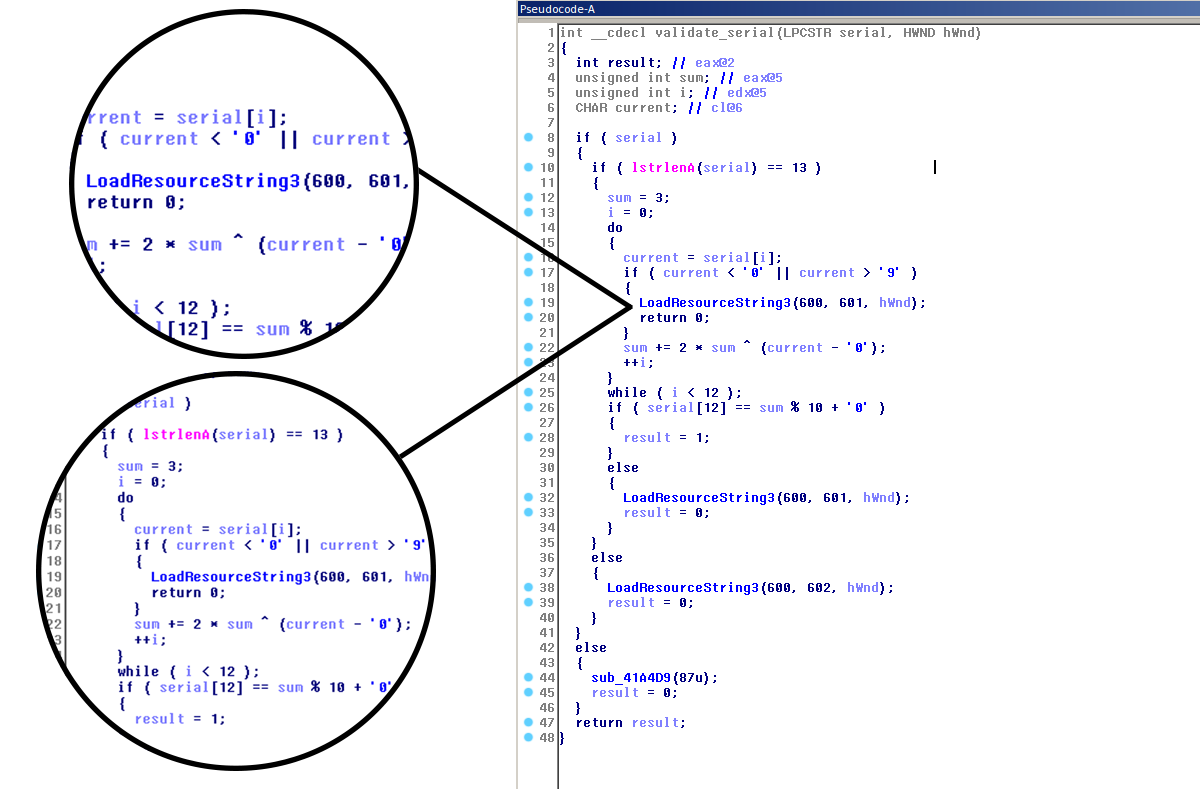
\includegraphics[width=\textwidth]{images/sc1-4-validator-rev-zoom.png}
\end{frame}

\begin{frame}{Getting to the core: Call graph}
	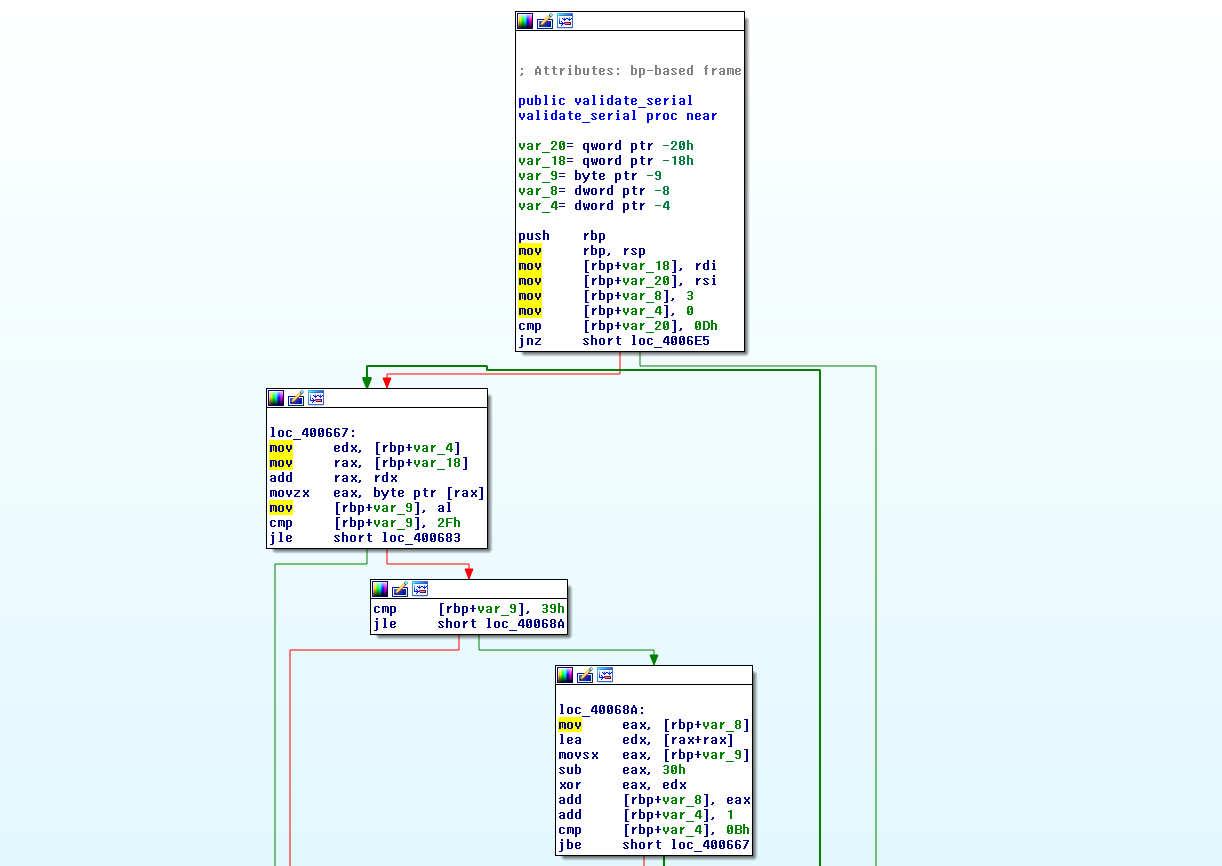
\includegraphics[width=0.9\textwidth]{images/sc1-5a-validator-graph.png}
\end{frame}

\begin{frame}{Getting to the core: Call graph}
	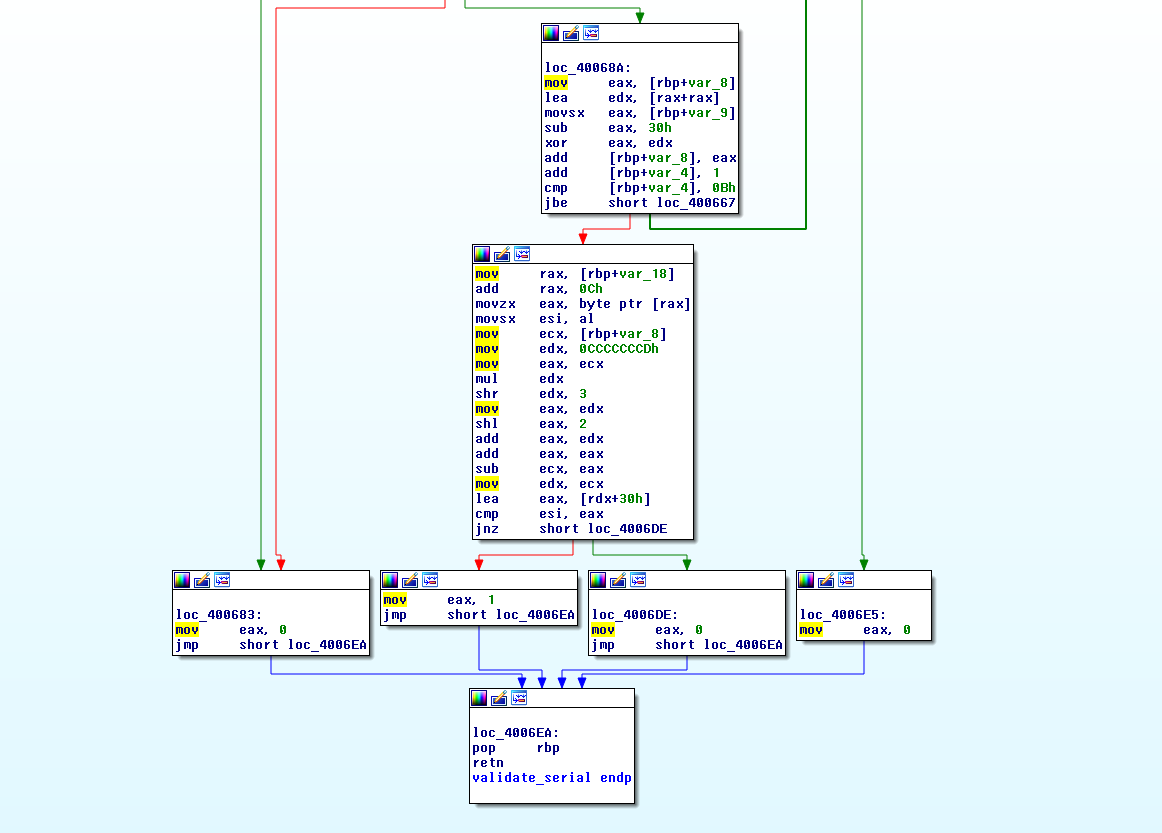
\includegraphics[width=0.9\textwidth]{images/sc1-5b-validator-graph.png}
\end{frame}

\begin{frame}{Getting to the core: Decompilation}
	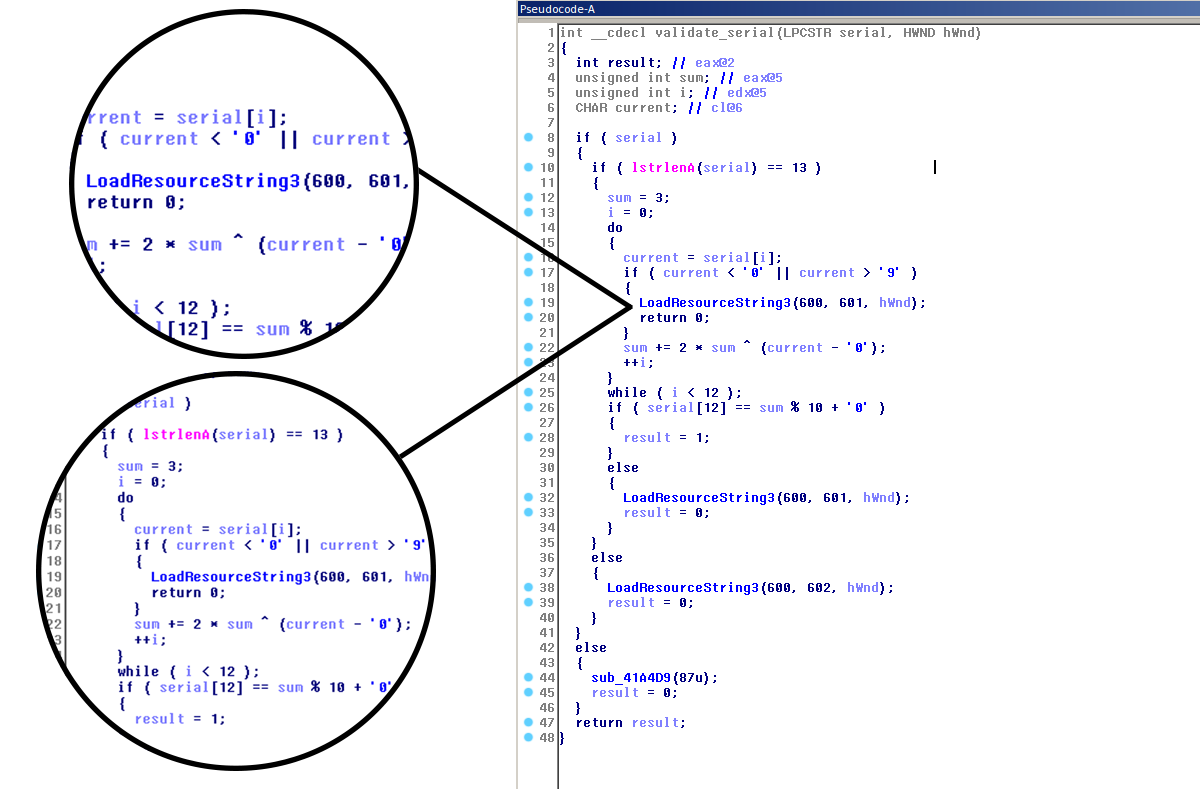
\includegraphics[width=\textwidth]{images/sc1-4-validator-rev-zoom.png}
\end{frame}

\begin{frame}{Z3: Formulating formulas}
	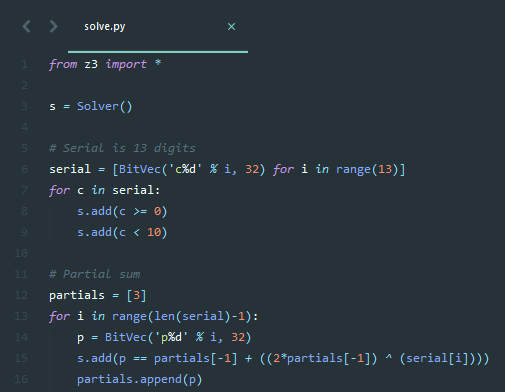
\includegraphics[width=0.85\textwidth]{images/sc1-6-z3-1.png}
\end{frame}

\begin{frame}{Z3: Formulating formulas}
	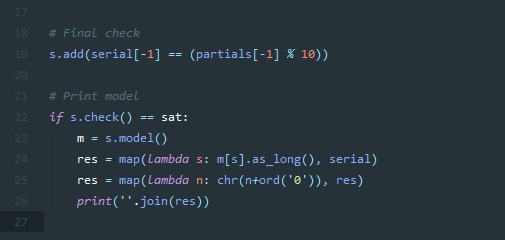
\includegraphics[width=0.85\textwidth]{images/sc1-6-z3-2.png}
\end{frame}

\begin{frame}{Once again, with fee... angr}

	\begin{columns}
		\begin{column}{0.7\textwidth}
	
		\begin{itemize}
		\item "python framework for analyzing binaries"
		\item "both static and dynamic symbolic (concolic)"
		\item Computer Security Lab at UC Santa Barbara
		\item Uses Z3 internally
		\end{itemize}
	\end{column}
		\begin{column}{0.3\textwidth}
			
\includegraphics[width=\textwidth]{images/angr-logo.png}
		\end{column}
	\end{columns}	

\end{frame}

\begin{frame}{Angr management: Extracting the code}
	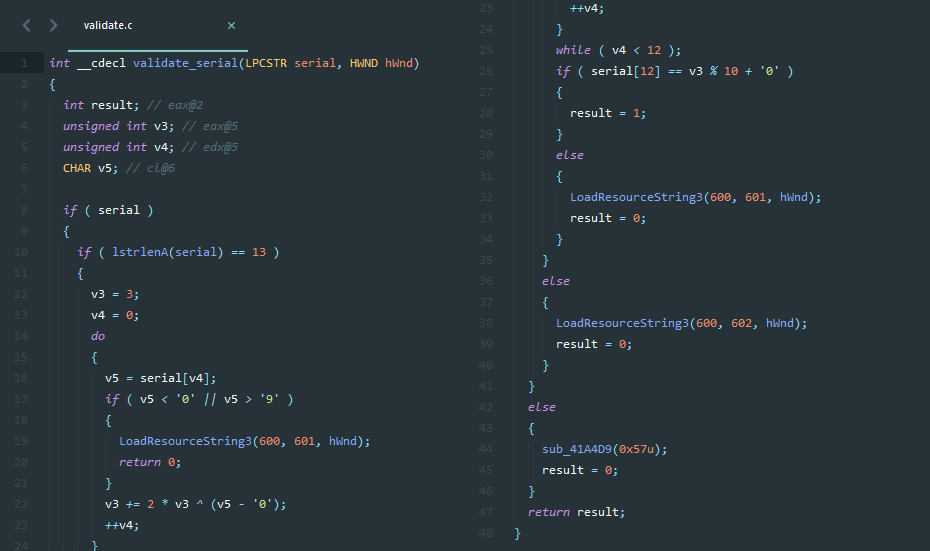
\includegraphics[width=\textwidth]{images/sc1-7-validator-split.png}
\end{frame}

\begin{frame}{Angr management: Minimizing the code}
	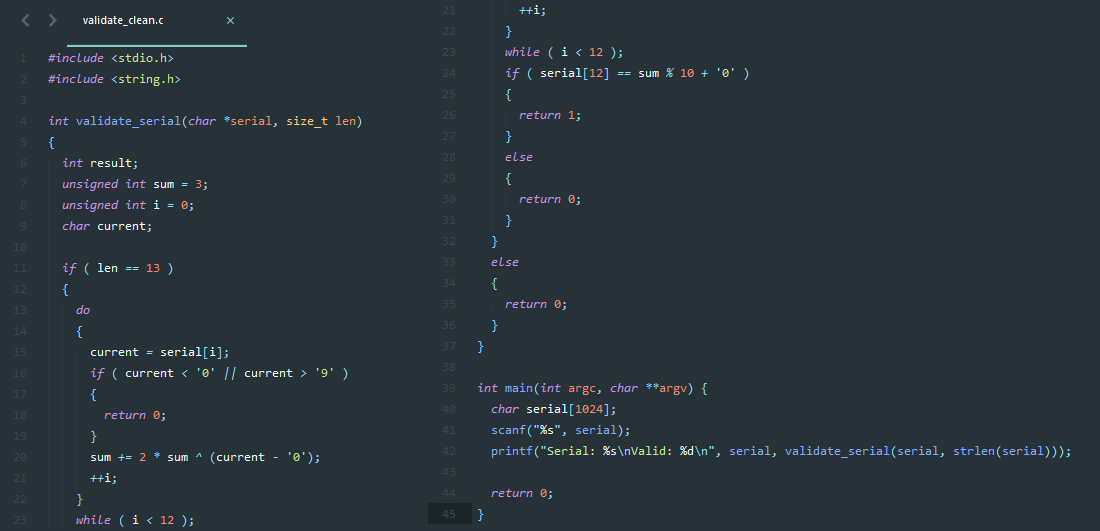
\includegraphics[width=\textwidth]{images/sc1-8-validator-clean-split.png}
\end{frame}

\begin{frame}{Angr management: Writing the explorer}
	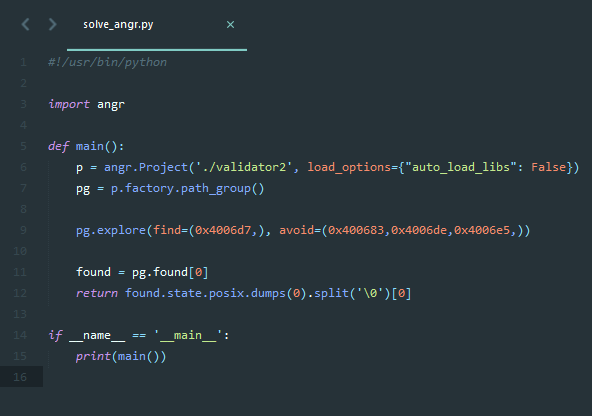
\includegraphics[width=0.90\textwidth]{images/sc1-9-angr.png}
\end{frame}



\plain{Thanks for listening!}

\end{document}
